\documentclass[conference]{IEEEtran}
\IEEEoverridecommandlockouts
% The preceding line is only needed to identify funding in the first footnote. If that is unneeded, please comment it out.
\usepackage{cite}
\usepackage{amsmath,amssymb,amsfonts}
\usepackage{algorithmic}
\usepackage{graphicx}
\usepackage{textcomp}
\usepackage{xcolor}
\usepackage{booktabs}                        % AAB inserido
\usepackage[utf8]{inputenc}                  % AAB inserido
\usepackage{rotating}                        % AAB inserido
%\usepackage{subfigure}                       % AAB inserido
%\usepackage[export]{adjustbox}               % AAB inserido

\ifCLASSOPTIONcompsoc                        % AAB inserido
\usepackage[caption=false,font=normalsize,labelfont=sf,textfont=sf]{subfig}
\else
\usepackage[caption=false,font=footnotesize]{subfig}
\fi
%\usepackage[round,sort,nonamebreak]{natbib}  % AAB inserido
%\usepackage[round,sort,nonamebreak]{natbib} % citação bibliográfica textual
\def\BibTeX{{\rm B\kern-.05em{\sc i\kern-.025em b}\kern-.08em
    T\kern-.1667em\lower.7ex\hbox{E}\kern-.125emX}}
%AAB
\DeclareMathOperator{\traco}{tr}
\graphicspath{{../../Dissertacao/figuras/}}
\begin{document}

\title{The edges evidence fusion to intensity channels in
PolSAR image\\
%{\footnotesize \textsuperscript{*}Note: Sub-titles are not captured in Xplore and
%should not be used}
\thanks{Grantee Capes/PROSUP/Mackenzie.}
}

\author{\IEEEauthorblockN{Anderson A. de Borba}
\IEEEauthorblockA{\textit{Dept.\ Engenharia Elétrica e Computação} \\
\textit{UPM -- Universidade Presbiteriana Mackenzie}\\
IBMEC, SP\\
São Paulo, Brazil \\
anderson.borba@ibmec.edu.br}
\and
\IEEEauthorblockN{Maurício Marengoni}
\IEEEauthorblockA{\textit{Dept.\ Engenharia Elétrica e Computação} \\
\textit{UPM -- Universidade Presbiteriana Mackenzie}\\
São Paulo, Brazil \\
mauricio.marengoni@mackenzie.br}
\and
\IEEEauthorblockN{\hspace{6cm} Alejandro C. Frery}
\IEEEauthorblockA{\textit{\hspace{6cm}Laboratório de Computação Científica e Análise Numérica -- LACCAN} \\
\hspace{6cm}\textit{UFAL -- Universidade Federal de Alagoas}\\
\hspace{6cm} Maceió, Brazil \\
\hspace{6cm}acfrery@gmail.com}
}

\maketitle

\begin{abstract}
There are different methods for detection and fusion of edge evidences in remote sensing. 
However, some of them, when applied to PolSAR images, produce inadequate results. 
%In order to improve the signal-to-noise ratio, there has been an investment in research with the use of statistical modeling. 
%%% ACF Junção de coisas inconexas
The present study proposes a method of detection and fusion of evidence edges based on the method of maximum likelihood, followed by fusion of information by average, SWT, PCA, and ROC statistics. 
We applied these techniques to the intensity channels of a PolSAR image. 
The results indicate a good performance of the method in detecting edges with possible paths for future research.
\end{abstract}

\begin{IEEEkeywords}
PolSAR, edge detection, maximum likelihood estimation, fusion
\end{IEEEkeywords}

\section{Introduction}\label{sec_01}

We present results on the detection and fusion of edge evidence applied to Polarimetric Synthetic Aperture Radar images (PolSAR). 
We employ models and algorithms as required for an appropriate treatment of their special characteristics~\cite{slf_2008}.

Among the available edge detection techniques for SAR imagery, it is worth mentioning those based on the gradient~\cite{tlb, obw, flmc, fyf}, and on Markov chains~\cite{bf}.
The former suffer from the effect of speckle noise, and the latter lead to computer intensive methods.

Ref.~\cite{gfn} presents a comparison between several edge detectors. 
Alternatively, techniques based on statistical modeling have been used in edge detection~\cite{gmbf, fbgm, horrit, gfn} and, more recently, by means of \textit{Deep Learning}~\cite{bac, ztmxzxf, tabmm, xstz}.

This work relies on ideas stemming from \textit{Information Fusion}.
This approach has been followed by Refs.~\cite{sglmla,sg} in order to extract valuable knowledge from remotely sensed data.

This paper will follow the statistical modeling approach, mainly the techniques described by~\cite{fbgm, nhfc} using the Wishart distribution. 
To perform the fusion of information we have as a basis Refs.~\cite{mit, sg}. 

The objective of this work is to detect edges in each channel of a PolSAR image and to perform the fusion of the edge evidence, with the task of understanding and of quantifying the importance of the information provided by each channel. 

The article is structured as follows: 
Section~\ref{sec_02} describes the statistical modeling for PolSAR data, 
it use is presented in Sections~\ref{sec_03}, \ref{sec_04} and~\ref{sec_05}.
Section~\ref{sec_06} describes the fusion of edge evidence approaches with an emphasis on the ROC statistics-based method.
Numerical results are shown and analyzed in Section~\ref{sec_07} and, finally, Section~\ref{sec_08} concludes the paper with remarks and future research directions.

\section{Statistical modeling for PolSAR data}\label{sec_02}

Fully polarimetric SAR systems transmit orthogonally polarized microwave pulses and measure orthogonal components of the received signal. 
For each pixel, we have a matrix of scattering coefficients, which are complex numbers and describe the transformation from the transmitted electromagnetic field to the received electromagnetic field.

The transformation can be represented as
\begin{equation*}
 \left[
\begin{array}{c}
	E_{h}^{r}   \\
	E_{v}^{r}    
\end{array}
\right]
 = \frac{e^{\hat{\imath} kr}}{r}\left[
\begin{array}{cc}
	S_{hh}   & S_{hv}   \\
	S_{vh}   & S_{vv}   
\end{array}
\right]
 \left[
\begin{array}{c}
	E_{h}^{t}   \\
	E_{v}^{t}    
\end{array}
\right],
\end{equation*}
where $k$ denotes the wave number, $\hat{\imath}$ is the complex unit, and $r$ is the distance between the radar and the target. 
The electromagnetic field with components $E_{i}^{j}$ has a subscribed index denoting horizontal ($h$) or vertical ($v$) polarization, while the superscript index indicates the received ($r$) or transmitted ($t$) wave. 
Defining $S_{i,j}$ as the complex scattering coefficients, such that the indexes $i$ and $j$ are associated with the reception and transmission of waves, for example, the scattering coefficient $S_{hv}$ is associated with wave transmitted in the vertical direction ($v$) and received in the horizontal direction ($h$).

Knowing each coefficient, the complex scattering matrix $\mathbf{S}$ is defined by
\begin{equation}\label{eq_01}
\mathbf{S} = \left[
\begin{array}{cc}
	S_{hh}   & S_{hv}   \\
	S_{vh}   & S_{vv}   
\end{array}
\right],
\end{equation}
and if the means of propagation of waves is reciprocal, then we will use the reciprocity theorem~\cite{lp} to define the scattering matrix as being Hermitian. 
In this way, the scattering matrix can be represented by the vector
\begin{equation}\label{eq_02}
\mathbf{s} = \left[
\begin{array}{c}
	S_{hh}     \\
    S_{hv}     \\
	S_{vv}    
\end{array}
\right].
\end{equation}

Following Refs.~\cite{good, lee}, we will assume that the distribution of $\mathbf{s}$ is circular Gaussian complex multivariate with zero mean $N^C_3(0,\Sigma)$, with probability density function (pdf) given by:
\begin{equation}
    f_{\mathbf{s}}(\mathbf{s};\mathbf{\Sigma})=\frac{1}{\pi^3|\mathbf{\Sigma}|} \exp(-\mathbf{s}^H\mathbf{\Sigma}^{-1}\mathbf{s}),
    \label{eq_03}
\end{equation}
where $|\cdot|$ is the determinant, 
the superscript index $H$ denotes the conjugate complex number, 
and $\mathbf{\Sigma}$ is the covariance matrix of the sample $\mathbf{s}$ such that $\mathbf{\Sigma}=E(\mathbf{ss}^H)$. 

As a result of the distribution being circular complex multivariate Gaussian with zero mean, and being the entries of $\mathbf{s}$ complex values $\mathbf{s}_{ij}= R_{ij}+ \hat{\imath} I_{ij}$, then $R_{ij}$ and $I_{ij}$ with $j=h,v$ satisfy:
\begin{itemize}
	\item[I-] $E[R_{ij}]=E[I_{ij}]=0$,
	\item[II-] $E[R_{ij}^2]=E[I_{ij}^2]$, 
	\item[II-] $E[R_{ij}I_{ij}]=0$,  
	\item[IV-] $E[R_{ij}R_{ij}]=E[I_{ij}I_{ij}]$, 
	\item[V-] $E[I_{ij}R_{ij}]=-E[R_{ij}I_{ij}]$,
\end{itemize}
where $E[cdot]$ denotes the expected value. 

This statistical modeling has been confirmed for a variety of targets for polarimetric SAR data, and it contains all the necessary information to characterize the backscatter~\cite{sarabendi,mfp}.
 
The statistical modeling described so far deals only with single-look modeling.
However, polarimetric images are usually subject to a multi-look processing in order to improve the ratio between the signal and the noise. 
For this purpose~\cite{good, ade}, estimated positive definite Hermitian matrices are obtained by computing the average of $L$ independent targets of the same scene, resulting in the estimated sample covariance matrix as:
\begin{equation}
    \mathbf{Z}=\frac{1}{L}\sum_{\ell=1}^{L} {\mathbf{s}_\ell}{\mathbf{s}_\ell}^H,
    \label{eq_04}
\end{equation}
where $\mathbf{s}_\ell$ with $\ell = 1, \dots, L$ are $L$ samples of complex vectors distributed as $\mathbf{s}$, so the sample covariance matrix associated with $\mathbf{s}_\ell$ denotes the scattering for each of the $L$ looks.

\section{Multi-look Wishart density function}\label{sec_03}
The multi-look process has the Wishart probability density function (pdf) defined by,
\begin{equation}\label{eq_05}
    f_{\mathbf{Z}}(\mathbf{Z};\mathbf{\Sigma_{s}},L)=\frac{L^{mL}|\mathbf{Z}|^{L-m}}{|\mathbf{\Sigma_{s}}|^{L}\Gamma_m(L)} \exp(-L\traco(\mathbf{\Sigma_{s}}^{-1}\mathbf{Z})), \\
\end{equation} 
where, $\traco(\cdot)$ is the trace operator of an array, $\Gamma_m(L)$ is a multivariate Gamma function defined by
\begin{equation*}
	\Gamma_m(L)=\pi^{\frac{1}{2}m(m-1)} \prod_{i=0}^{m-1}\Gamma(L-i) \\
\end{equation*}
and $\Gamma(\cdot)$ is the Gamma function and $m=3$ for the present article. It can be said that $\mathbf{Z}$ is distributed as a Wishart distribution denoting for $\mathbf{Z}\sim W(\mathbf{\Sigma_{s}}, L)$ and satisfying $E[\mathbf{Z}]=\mathbf{\Sigma_{s}}$. Without loss of generality to the text, let is use the symbol $\mathbf{\Sigma}$ instead of $\mathbf{\Sigma_{s}}$ to represent the covariance matrix associated with $\mathbf{S}$.

\section{Edge Detection}\label{sec_04}
In the specialized literature, it is found a large offer of classical methods to detect edge, for example, Sobel, Canny, Laplacian da Gaussian (LoG) and LoG pyramidal. The classical edge detection methods are constructed assuming that noise is additive, which makes these methods inefficient for application in PolSAR images.

Based on the articles \cite{nhfc, gmbf}, it is possible to propose an edge detection method for PolSAR images with multiple targets.The main idea is to detect the transition point in a thin a range, as possible, between two regions of the image. The transition point is defined as edge evidence. The noise in these types of images is the \textit{speckle} type, and has multiplicative nature, making edge detection in SAR images a challenging task.

Edge detection methodologies occur in several stages, as follows:
\begin{enumerate}
	\item identify the centroid of a region of interest (ROI) in an automatic, semi-automatic or manual manner;
	\item to build centroid rays out of the area of interest;
	\item to collect data on a neighbourhood around the rays using the {\it Bresenham's midpoint line algorithm}, ideally the size of a pixel;
	\item detect points in the data range, which provide evidence of statistical property changes, i.e., a transition point that defines border evidence;
	\item use the Generalized Simulated Anneling (GenSA) method, reference \cite{xgsh}, to find maximum points in functions of interest;
	\item fusion of evidence of detected edges in $(hh)$, $(hv)$ and $vv$ channels.
\end{enumerate}

\section{Maximum Likelihood Method}\label{sec_05}
The Maximum Likelihood Estimation (MLE) is a method estimates the parameters values of the model maximizing the data probability function, considering as known a data set and a statistical model. More details on the likelihood concept can be found in \cite{nhfc, gmbf}.

Suppose $\mathbf{X}=(X_1,X_2,\dots,X_n)^T$ a random vector distributed according to the probability density function (pdf) $f(\mathbf{x},\mathbf{\theta})$ with parameters $\mathbf{\theta}=(\theta_1,\dots,\theta_d)^T$ in the parameter space $\Theta$, it is defined the likelihood function  
\begin{equation*}
    L(\theta;\mathbf{X}) = \prod_{i=1}^{n}f(x_i;\theta), \\
\end{equation*}
and the logarithmic likelihood function, which is also called the log-likelihood function
\begin{equation}\label{eq_09}
	l(\theta;\mathbf{X})= \ln(L(\theta;\mathbf{X})) = \sum_{i=1}^{n}\ln(f(x_i;\theta)). \\
\end{equation}

In a simplified form, the estimate of maximum likelihood can be written by 
\begin{equation*}
    \widehat{\theta}= \text{arg}\,\max\limits_{\theta\in\Theta}L(\theta;\mathbf{x}),\\
\end{equation*}
and similarly
\begin{equation*}
    \widehat{\theta}= \text{arg}\,\max\limits_{\theta\in\Theta}l(\theta;\mathbf{x}).\\
\end{equation*}

Using the maximum likelihood method applied to the Wishart distribution, suppose $\mathbf{Z}=(\mathbf{Z}_1,\mathbf{Z}_2,\dots,\mathbf{Z}_N)^T$ a random vector distributed according to the probability density function (pdf) (\ref{eq_05}) with parameters $\Sigma=\{\mathbf{\Sigma_A}, \mathbf{\Sigma_B}\}$ and $L$. The parameters $\mathbf{\Sigma_A}$, $\mathbf{\Sigma_B}$ belong to two different samples $A$ and $B$, and the goal is to detect the border between the two samples.

The likelihood function of the sample described by (\ref{eq_09}) is given by the production equation of the density functions, respectively associated to each sample.
\begin{equation}\label{eq_10}
	L(j)=\prod_{k=1}^{j}f_{\mathbf{Z}}(\mathbf{Z}_{k}^{'};\mathbf{\Sigma_{A}},L) \prod_{k=j+1}^{N}f_{\mathbf{Z}}(\mathbf{Z}_{k}^{'};\mathbf{\Sigma_{B}},L), \\
\end{equation}
where $\mathbf{Z}_{k}^{'}$ is a possible approximation of the random matrix described in (\ref{eq_04}).

Using the equation (\ref{eq_09}), one has the log-likelihood function.
\begin{equation}
\begin{array}{rcl}\label{eq_11}
	l(j)=\ln L(j)&=&\sum_{k=1}^{j}\ln f_{\mathbf{Z}}(\mathbf{Z}_{k}^{'};\mathbf{\Sigma_{A}},L)\\
	             &+&\sum_{k=j+1}^{N}\ln f_{\mathbf{Z}}(\mathbf{Z}_{k}^{'};\mathbf{\Sigma_{B}},L).
\end{array}
\end{equation}

At this moment, we can perform algebraic manipulations in the probability density function in each term of the summation and replace in the two parts of the equation (\ref{eq_09}) resulting in
\begin{equation}
\begin{array}{lll}\label{eq_12}
	l(j)&=&N\left[mL\ln{\left(L\right)}-\ln{\left(\Gamma_m(L)\right)}\right]\\
	&-& L\left[j\ln{\left(|\mathbf{\Sigma_{A}}|\right)}+(N-j)\ln{\left(|\mathbf{\Sigma_{B}}|\right)}\right] \\
	&+&(L-m)\sum_{k=1}^{N}\ln{\left(|\mathbf{Z}_{k}^{'}|\right)}\\
	&-&L\left[\sum_{k=1}^{j}tr(\mathbf{\Sigma_{A}}^{-1}\mathbf{Z}_{k}^{'})+ \sum_{k=j+1}^{N}tr(\mathbf{\Sigma_{B}}^{-1}\mathbf{Z}_{k}^{'})\right]. \\
\end{array}
\end{equation}

The $\Sigma$ matrix can be found using the maximum likelihood estimator denoted by $\widehat{\Sigma}$ according to the reference \cite{good}. The equation (\ref{eq_13}) represents two estimates for the covariance matrix $\Sigma$ that depend on the $j$ position.
\begin{equation}\label{eq_13}
\widehat{\Sigma_{I}}(j) = \left\{
\begin{array}{lc}
	j^{-1}\sum_{k=1}^{j}\mathbf{Z}_{k}  & \mbox{se}\quad I=A,  \\
        (N-j)^{-1}\sum_{k=j+1}^{N}\mathbf{Z}_{k} & \mbox{se}\quad I=B. \\
\end{array}
\right.
\end{equation}

In the equation (\ref{eq_12}) we can replace the equation (\ref{eq_13}) and continue the algebraic manipulation, resulting in 
\begin{equation}\label{eq_14}
\begin{array}{rcl}
	l(j)&=&N\left[-mL(1-\ln{L)})-\ln{\left(\Gamma_m(L)\right)}\right]\\
	&-&L\left[j\ln{|\mathbf{\widehat{\Sigma}}_{A}(j)|} +(N-j)\ln{|\mathbf{\widehat{\Sigma}}_{B}(j)|}\right]\\
	&+&(L-m)\sum_{k=1}^{N}\ln{|\mathbf{Z}_{k}^{'}|}. \\
\end{array}
\end{equation}

The maximum argument $\widehat{\jmath}_{ML}$ is edge evidence that will be used in fusion methods.
\begin{equation*}
\begin{array}{rcl}
	\widehat{\jmath}_{ML}&=&\text{arg}\max\limits_{j}l(j).  \\
\end{array}
\end{equation*}
\section{Methods of fusion of border evidence}\label{sec_06}
\subsection{Simple mean}
The simple mean fusion method proposes the arithmetic mean of the edge evidence in each channel. The edge evidence fusion can be calculated by
\begin{equation}
	IF(x,y)=\frac{1}{nc}\sum_{i=1}^{nc}IE_i(x,y),
\end{equation}
where $nc$ is the number of channels to be used in the fusion. We can get more details on the reference \cite{mit}.
\subsection{Stationary wavelet transform- SWT} 
This section is again based on the reference \cite{n_r}. The SWT fusion method can be described by the following steps:
\begin{itemize}
\item[-] calculate the SWT decomposition by getting $L_{HH}$, $L_{HL}$, $L_{LH}$ and $L_{LL}$ for each channel;
\item[-] in the decompositions $L_{HH}$ the arithmetic mean of all channels, pixel by pixel, and in the decompositions $L_{HL}$, $L_{LH}$ and $L_{LL}$ is performed, is found the maximum between each channel, pixel by pixel, leaving a new decomposition $\bar{L}_{HH}$, $\bar{L}_{HL}$, $\bar{L}_{LH}$ and $\bar{L}_{LL}$;
\item[-] performing the reverse transformation of SWT, we get the image by fusing the edge evidence $IF(x,y)$.  
\end{itemize}

\subsection{Pincipal component analysis - (PCA) }
This section is based on \cite{n_r} and \cite{mit}, where the PCA-based fusion method can be described by the following steps:
\begin{itemize}
\item[-] organize the data in such a way that each image has a column vector, forming a $Y$ matrix of dimension $l\times nc$, where $l=m\cdot n$, represents the multiplication of $m$ lines and $n$ columns of the matrices to be used in the fusion;
\item[-] calculate the average of the elements of these columns, generating a vector dimension of $1\times nc$;
\item[-] subtract the average of each column from the $Y$ matrix. Resulting in a $X$ matrix of the same dimension of $Y$; 
\item[-] find the $C$ covariance matrix from $X$, calculating $C=XX^T$;
\item[-] calculate the eigenvalues $\Lambda$ and the eigenvectors $D$, and sort the eigenvalues and eigenvectors in descending order. The matrices generated by the eigenvalues, on the main diagonal, and the eigenvectors placed in column, have dimensions $nc\times nc$;
\item[-] compute the components $P_i=\frac{V_i}{\sum_{i=1}^l V_i}$ with $i=1,\dots,nc$;
\item[-] we fuse $IF(x,y)=\sum_{i=1}^{nc}P_iIE_i(x,y)$. Remembering that the $\sum_{i=1}^{nc}P_i=1$.
\end{itemize}

\subsection{ROC statistics}
The ROC statistical method was proposed and described in detail in the references \cite{gs} and \cite{fawcett}. The method describes a statistical model to obtain information automatically, from several images, or in several channels. The method can be described in the following procedures:
\begin{itemize}
\item[-] obtain the evidence of edges in the channels, applying the method described in this article. Store this edge evidence in $E_i$ matrices, with $i=1,\cdots,nc$ in a binary way;
\item[-] define a $V$ edge frequency matrix. The $V$ matrix is generated by adding the evidence of $E_i$ borders;
\item[-] use thresholds ranging from $t=1,\dots,nc$ generating $M_t$ matrices;
\item[-] compare each $M_t$, fixed with all $E_i$, find the confusion matrix to generate the ROC curve. The point of the ROC curve that approaches (in the sense of the Euclidean distance) the diagnostic line, will have its threshold considered optimal;
\item[-] the $M_t$ matrix, which corresponds to the threshold closest to the diagnostic line, is the fusion of edge evidence.
\end{itemize}

\section{Numerical results}\label{sec_07}
The PolSAR image, with 4 looks of the Flevoland region in the Netherlands, was used for the numerical tests. The figure (\ref{fig_01}) shows the region of interest, where it was built the radial lines for edge detection.

 Edge detection and subsequent evidence fusion were performed in this region of interest, in order to understand the weighting of each channel in the image formation.

In this study, edge detection was performed in the intensity channels (hh), (hv) and (vv), and subsequently, used for information fusion. 

%\begin{figure}[hbt]
%\centering
%	\includegraphics[scale=0.3]{flevoland_4_look.pdf}
%	\vspace{-1.0cm}
%		\caption{Imagem de Flevoland com 4 visadas.}
%\label{cap_acf_fig10}
%\end{figure}
\begin{figure}[hbt]
\centering
	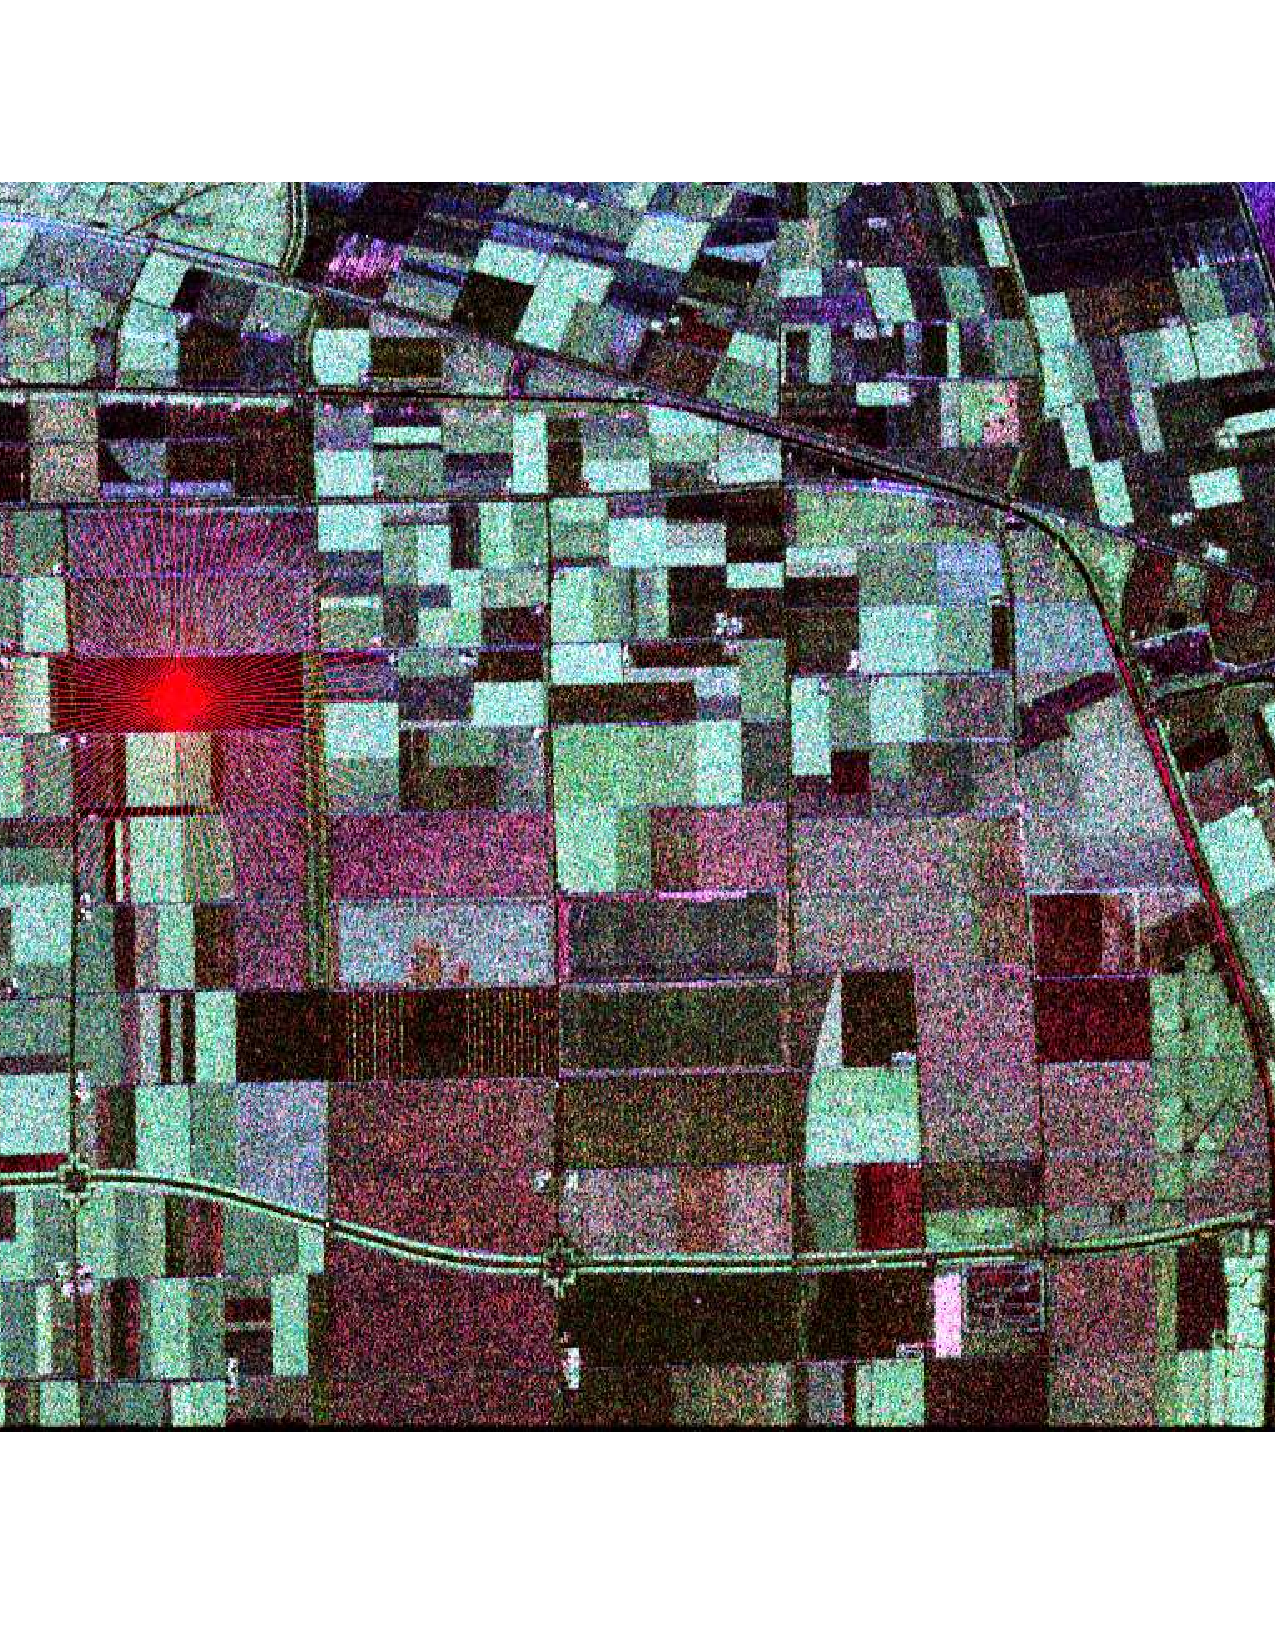
\includegraphics[scale=0.3]{flevoland_radial_4_look.pdf}
	%	\includegraphics[scale=0.3]{flevoland_radial_4_look.ps}
			\vspace{-1.0cm}
	\caption{Region of interest (ROI) in the image of Flavoland.}
\label{fig_01}
\end{figure}
The figures \ref{fig_02} \subref{fig:1a}, \subref{fig:1b} and \subref{fig:1c} show, respectively, the edge evidence detection algorithms, applied to (hh), (hv) and (vv) channels. 

The algorithm to detect evidence of edges worked well in the channels (hh) and (hv), achieving better accuracy in relation to the channel (vv).  

In the canal (vv), edges that are not part of the homogeneous region of interest were detected, but are part of other edges of the image, researching the reason for this fact, we analyzed the function $l(j)$ and found that the function presents two peaks, representing possible evidence of edges, in which the largest was correctly detected. 



   \begin{figure}[!ht]
     \subfloat[Evidence in channel (hh) \label{fig:1a}]{%
       %\includegraphics[width=0.2\textwidth]{example-image-a}
       \includegraphics[width=0.2\textwidth]{flevoland_hh_evid_crop_teste.pdf}       
     }
     \hfill
     \subfloat[Evidence in channel (hv) \label{fig:1b}]{%
       \includegraphics[width=0.2\textwidth]{flevoland_hv_evid_crop_teste.pdf}
     }
     \\
     \centering
     \subfloat[Evidence in channel (vv) \label{fig:1c}]{%
       \includegraphics[width=0.2\textwidth]{flevoland_vv_evid_crop_teste.pdf}
     }
     \caption{Dummy figure}
     \label{fig_02}
   \end{figure}

The figures \ref{fig_03} \subref{d} to \subref{g} show, respectively, the fusion of evidence for the methods described in this article. In order, we list the method that shows the average of edge evidence, the method that uses the Stationary wavelet transform (SWT), the method that uses the Principal component analysis (PCA), and finally, the method based on ROC statistics.

The methods shown in the figures \ref{fig_03} \subref{d}, \subref{e} and \subref{f} use all the pixels detected in the different channels. Each method weighs the pixels in the different channels with their characteristics. The average also weighs the pixels. The (SWT) finds the coefficients of the linear combination of its wavelet bases, and the (PCA) weights the auto-vectors of the covariance matrix.

The ROC statistics method does not use all pixels of the channels, because the method is based on thresholds discarding pixels. This was observed in the figure \ref{fig_03}\subref{g}.

\begin{figure}[!ht]
     \subfloat[Fusion media\label{d}]{%
       %\includegraphics[width=0.2\textwidth]{example-image-a}
       \includegraphics[width=0.2\textwidth]{flevoland_fusao_media_crop_teste.pdf}       
     }
     \hfill
     \subfloat[Fusion SWT\label{e}]{%
       \includegraphics[width=0.2\textwidth]{flevoland_fusao_swt_crop_teste.pdf}
     }
     \\
     \subfloat[Fusion PCA\label{f}]{%
       %\includegraphics[width=0.2\textwidth]{example-image-a}
       \includegraphics[width=0.2\textwidth]{flevoland_fusao_pca_crop_teste.pdf}       
     }
     \hfill
     \subfloat[Fusion ROC\label{g}]{%
       \includegraphics[width=0.2\textwidth]{flevoland_fusao_roc_crop_teste.pdf}
     }
     \\
     %\centering
     %\subfloat[First sub-figure\label{flevoland_vv_evid_crop.pdf}]{%
     %  \includegraphics[width=0.2\textwidth]{flevoland_hv_evid_crop_teste.pdf}
     %}
     \caption{Dummy figure}
     \label{fig_03}
   \end{figure}

\section{Conclusion}\label{sec_08}
In this study, the statistical modelling approach was applied to real PolSAR data imaging. Aiming to understand the importance of information from each channel in the edge evidence fusions, the proposed algorithm was applied in three intensity channels (hh), (hv) and (vv). Initially, it was found the evidence of edges, using the maximum likelihood  method in each channel, obtaining good results. After analyzed the results obtained in the three channels, it was observed that the method for the edge detections worked better in the channels (hh) and (hv) than the channel (vv), achieving a suitable accuracy.

Subsequently, the fusion of evidence of edges was performed with the methods of simple mean, SWT, PCA and ROC statistics. The first three methods performed well as shown in the results. The ROC statistics method suppressed several edge points, a behaviour expected because it is a method that uses thresholds; however, when applied in a larger number of channels, its performance tends to improve. 

Based on these results, a possible way to improve them would be to increase the number of channels studied. This analysis open a way for future researches with application of different methods for edge evidence fusing.
\bibliographystyle{IEEEtran}
\bibliography{bibliografia}
\end{document}
